\chapter{METODOLOGIA}

%Metodologia da bibliografia

Este estudo se apresenta como um trabalho de pesquisa quantitativa exploratória de conteúdos assim como de estudo de caso, a metodologia utilizada para o desenvolvimento do estudo estará estruturada em três fases: 

\begin{itemize}
    \item Revisão sistemática dos conteúdos bibliográficos e documentais;
    \item Desenvolvimento do Modelo conceitual para Transferência de Tecnologia Agrícola;
    \item Validação do Modelo Proposto;
\end{itemize}

\section{Revisão sistemática dos conteúdos bibliográficos e documentais}

Para atingir os objetivos que orientam este estudo, os procedimentos metodológicos foram idealizados com base em pesquisas anteriores que visam o desenvolvimento de novos modelos teóricos para melhoria da gestão de tecnologias, em instituições de ensino públicas e particulares, como também Centros de pesquisa. 

A metodologia de revisão sistemática dos textos acadêmicos utilizada encontra-se esquematizada na Figura \ref{figura_29}. 

\begin{figure}[H]
\centering
\caption{\textbf{Planejamento da Revisão Sistemática dos textos acadêmicos}}
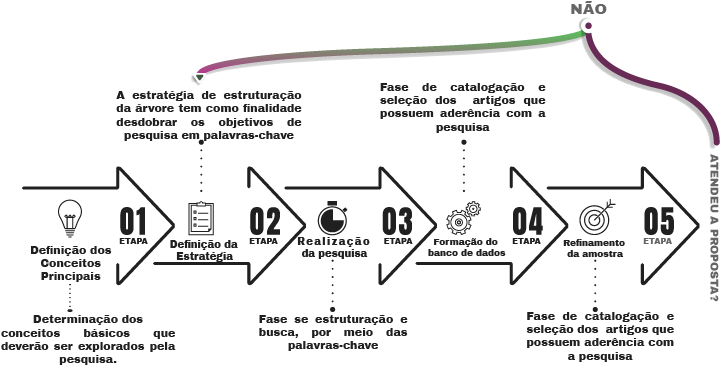
\includegraphics[scale=0.6]{Imagens/fases_pesquisa_bibliografica.png}
\fonte{Adaptado de \citeonline{fao_panorama_2017}}
\label{figura_29}
\end{figure}


Será realizada uma busca dos descritores que serão utilizados inicialmente, para isto serão prospectadas as bases de dados bibliográficos \textit{Scorpus} e \textit{IEEE Xplore} visando selecionar os artigos científicos e materiais didáticos relacionados ao tema.

Objetivando vincular as fontes de consulta com o tema proposto, serão adotados como descritores primários os termos: \textit{Technology Transfer}, \textit{Educational Institution} e \textit{Agriculture}, tendo como corte temporal o intervalo entre 2014 e 2020. 

Partindo dos corpus textuais selecionados, os descritores foram categorizados através do software VOSviewer. O método consiste em um agrupamento textual, fazendo com que as palavras que façam mais sentido formem um número k de grupos, regidos por z centroides, em que um centroide é um termo que reproduz o eixo central de um grupo, quando observado um determinado tema. Desta forma, foram selecionados os principais descritores agrupados a cada \textit{cluster} observado. 


A revisão textual para o desenvolvimento dos conteúdos abordados no trabalho tem por objetivo construir os \textit{clusters} que deverão estar relacionados intimamente aos descritores primários utilizados (Tabela \ref{tabela_2}). 



A partir do desenvolvimento dos clusters e seus respectivos descritores principais, será desenvolvido uma nova busca nos bancos de dados anteriormente citados (\textit{Scorpus} e \textit{IEEE Xplore}), afinando assim os materiais a serem utilizados. No terceiro momento, buscando construir um referencial bibliográfico mais sólido sobre os conteúdos pretendidos neste estudo, será realizada uma revisão por classificação da importância e da situação de semelhança como ferramenta StArt (\textit{State of the Art through Systematic Review}) \cite{LaPES2005StArtSoftware}, seguindo o protocolo baseado nas orientações de \citeonline{Kitchenham2009SystematicReview}. 

Esta ferramenta (StArt) foi desenvolvida para apoiar todo processo de Revisão Bibliográfica, por meio de uma árvore hierárquica, categorizando os artigos em proximidade e níveis de aderência às palavras-chave \cite{Hernandes2010AvaliacaoGQM}.


\subsection{}{Levantamento dados sobre Transferência de Tecnologia}

\subsection{Raspagem dos Dados}

Os dados sobre transferência de tecnologias desenvolvidas pelos órgãos públicos direcionadas ao setor agrícola serão selecionados a partir das publicações disponíveis no Diário Oficial da União DOU.

Para delimitar o ambiente de estudo, serão adotados como indicadores os termos “Transferência de tecnologia*” e “Agricultura/Agrícola”. 

Como linha temporal serão selecionados os comentários realizados de 2016 a 2020. dos órgãos a serem pesquisados como Universidades públicas, Centros de Pesquisa e Empresas públicas.

Objetivando preservar a identidade das empresas envolvidas neste estudo, estas serão descritas como: (UP) Universidade Pública, (CP) Centro de Pesquisa, (EP) Empresa pública. Nesta fase do  estudo, será configurada, para a coleta automatizada, a raspagem utilizando a linguagem Python com o auxílio do Pandas para carregar os textos e armazenar as informações extraídas. A extração de informações será feita utilizando a biblioteca do IBM Watson em Python que permite o acesso aos serviços de Natural \textit{Language Understanting}.

Será utilizado o sistema Crawler programado para extrair os comentários sobre a percepção da estadia, desta forma, o processo de extração será realizado em cinco passos, a saber: acesso ao site de ofertas; paginação dos locais de hospedagem; loop de raspagem dos itens; extração dos dados e abertura de novas páginas. Este processo está representado  na Figura \ref{figura_raspagem}. Durante a coleta dos dados, as publicações que se mostraram em duplicidade serão suprimidas. 



\begin{figure}[H]
\centering
\caption{\textbf{Espaço de trabalho para raspagem de publicações no Diário Oficial da União sobre transferência de tecnologia agrícola}}
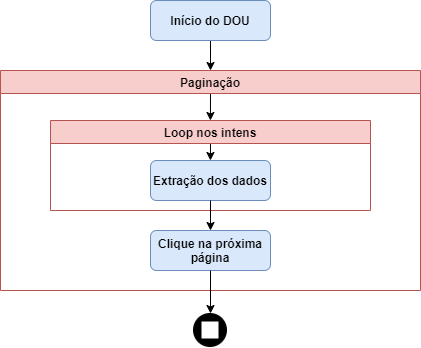
\includegraphics[scale=0.6]{Imagens/raspagem.png}
\fonte{Os Autores 2020.}
\label{figura_raspagem}
\end{figure}


\subsection{Análise quantitativa de dados textuais selecionados}

Após a seleção dos comentários diretamente relacionados ao tema proposto nesta pesquisa, serão realizadas lexicométricas e análises de discursos nos textos presentes com o auxílio do software IRaMuTeQ \cite{conde_lexicometria_2015,da_silva_cezar_panorama_2018}. Através da utilização de Unidades de Contexto Iniciais (UCIs) na construção do modelo para análise, será realizada uma prévia correção no conjunto de dados brutos mantendo as palavras analisáveis, os termos caracterizados como substantivos, adjetivos e verbos. As palavras que geralmente não são relevantes para uma análise, como preposições e advérbios, serão excluídas.

Ao se trabalhar com corpus textuais cada conjunto de texto deve compor uma UCI. Um conjunto de UCI é conhecido como corpus de análise, os quais o software segmenta em textos de aproximadamente três linhas, chamados de Segmento de Texto (ST) \cite{Fernandes2018AvaliacaoNatal/RN}. Após a segmentação dos textos, o software realiza uma Categorização Hierárquica Descendente (CHD) dando origem a classes lexicais caracterizadas pelo vocabulário e a segmentos de textos que partilham o mesmo vocábulo.

A Classificação Hierárquica Descendente (CHD) consiste em um tipo de análise de conglomerado que categoriza as palavras obtidas em classes lexicais (eixos). A análise avalia a constância e os arranjos das palavras ativas que estão no corpus textual usando os dados das tabelas de contingência das palavras existentes \cite{Carvalho2020UtilizacaoSanitaria,Mendes2019MappingAnalysis}. Neste sentido, as diferentes classes resultantes representam o espaço de sentido das palavras narradas, surgindo, assim, elementos pertencentes aos temas observáveis da pesquisa \cite{Gavasso2016RevisaoTreinamento}. 

Por fim, é importante ressaltar que a avaliação da metodologia proposta neste estudo será mediada pela técnica desenvolvida por \citeonline{Costa2015ConstrucaoSistematicas} tendo como base a \textit{Assessment of Multiple Systematic Reviews} (AMSTAR).


\section{Desenvolvimento do Modelo conceitual para Transferência de Tecnologia Agrícola}

\subsection{Dimensões consideradas no modelo}


Para o desenvolvimentos dos parâmetros que compõem o modelo preliminar que será analisado pelo método Delphi, serão consideradas cinco dimensões:

\begin{multicols}{2}
\centering
    \begin{itemize}
    \item{Pessoais atingidas pela Tecnologia;}
\item{Orçamento destinado a Transferência;}
\item{Relacionamento com a comunidade;}
\item{Gestão integrada da Tecnologia;}
\item{Propriedade Intelectual Resultante;}
\item{Potencial Validação;}
\item{Comercialização;}
\item{Responsabilidade Social;}
\item{Pesquisa e Desenvolvimento aplicado;}
\item{Sustentabilidade ambiental}
\end{itemize}
\end{multicols}


O modelo de transferência de tecnologia será embasado pelos modelos de \citeonline{Baek2007ANegotiations}, \citeonline{Bozeman2000TechnologyTheory} e \citeonline{Silva2016ModeloBrasileiros}. Os mesmos serão escolhidos pela sua estruturação no modelo e por serem mais citados na literatura.

Após a análise dos resultados da prospecção bibliográfica e  quantitativa de dados textuais será desenvolvido um questionário contendo questões relativas as dimensões citadas, que será aplicado aos juízes tendo como base o Método Delphi. O questionário ao final fara parte estrutural do modelo proposto neste experimento. Estas perguntas serão estruturadas seguindo uma escala Likert com perguntas de peso mínimo 1 e ao máximo 5. 


\section{Validação do Modelo Proposto}


Buscando mensurar a eficácia do modelo estudado nesta pesquisa, será utilizado o método Delphi como parâmetro de validação. Esta técnica consiste em buscar um senso comum do grupo de juízes, ou seja, profissionais efetivamente engajados na área de estudo. O método Delphi se baseia na aplicação estruturada do conhecimento e da experiência de especialistas da área pressupondo que, o julgamento em conjunto de determinado processo quando organizado adequadamente, é melhor que a opinião de um só indivíduo \cite{Faro1997TecnicaEnfermagem,Santiago2012MatrizUrbanos}.

Nela  ocorre uma estrutura de comunicação sistemática, controlada pelo pesquisador, permitindo que os juízes recebam \textit{feedbacks} acerca das opiniões expostas, recolocando suas opiniões e respondendo às entradas dos demais participantes, permitindo que, ao final das rodadas, se alcance o consenso do problema em questão \cite{Massaroli2017MetodoEnfermagem}. 

Na Figura \ref{figura_delphi} apresenta o movimento do questionário para o desenvolvimento do modelo de transferência de tecnologia, para tanto, serão convidados profissionais com expertise na área de produção tecnológica para agricultura, políticas públicas, transferência de tecnologia e agricultura sustentável. 

Além da vantagem de se ter profissionais notórios na área de pesquisa & inovação, o método Delphi apresenta a  possibilidade de inclusão de juízes de vários estados brasileiros, favorecendo desta forma o desenvolvimento da pesquisa e evitando assim o enviesamento causado pela presença de participantes de apenas uma região do Brasil, tornando assim o modelo final que será alcançado ao final da pesquisa, aplicável em todo o território nacional.


\begin{figure}[H]
\centering
\caption{\textbf{Movimento desenvolvido para operacionalização do método Delphi e a articulação das
abordagens}}
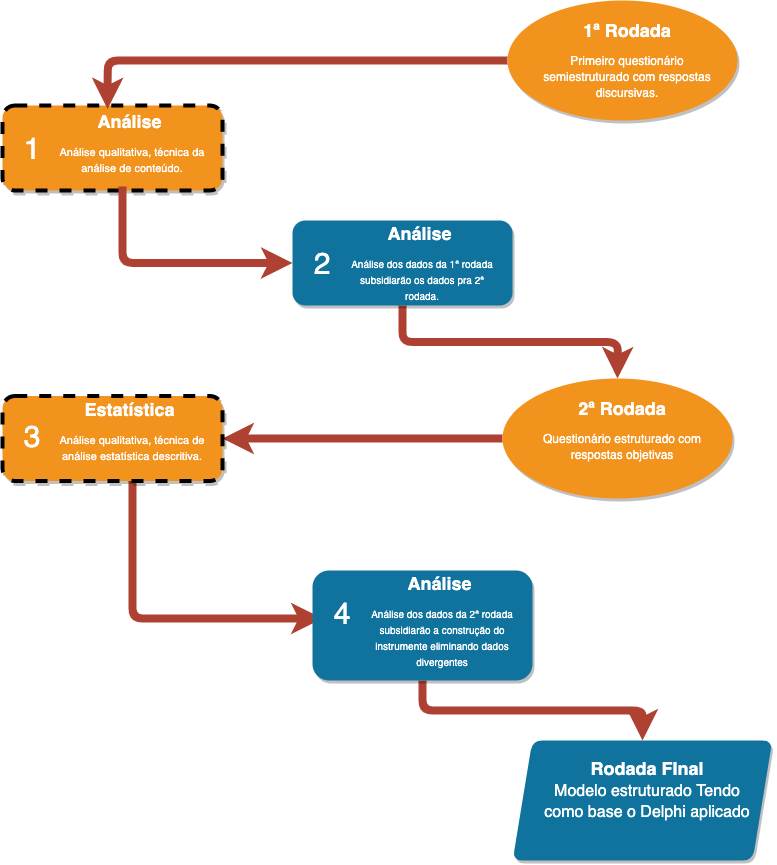
\includegraphics[scale=0.3]{Imagens/delphi.png}
\fonte{O Autor adaptado de \cite{massaroli_metodo_2017}}
\label{figura_delphi}
\end{figure}

A avaliação dos questionários aplicados ao  juízes será conduzida às cegas, desta forma, Acredita-se que o sigilo dos participantes garanta ao final do experimento uma maior fidelidade ao resultado, e permitindo ainda a estes uma melhor exposição dos resultados e a sustentação de seu ponto de vista sobre o modelo de transferência de tecnologia agrícola \cite{Keeney2011TheResearch}.